\documentclass[12pt, a4paper]{book}

\usepackage[T1]{fontenc}
\usepackage[utf8]{inputenc}
\usepackage[charter, cal=cmcal]{mathdesign}
\usepackage[scaled=0.92]{helvet}
\usepackage{geometry}
\geometry{a4paper, top=30mm, bottom=30mm, inner=32mm, outer=25mm, marginparwidth=18mm}

\usepackage{amsmath, amsthm}
\usepackage[version=4]{mhchem}
\usepackage{graphicx}
\usepackage{xcolor}
\usepackage{tikz}
\usetikzlibrary{arrows.meta, shapes.geometric, positioning, calc, backgrounds}
\usepackage{pgfplots}
\pgfplotsset{compat=1.18}
\usepackage{tcolorbox}
\tcbuselibrary{skins, breakable, theorems}
\usepackage{titlesec}
\usepackage{fancyhdr}
\usepackage{enumitem}
\usepackage{booktabs}
\usepackage{array}
\usepackage{parskip}
\usepackage{siunitx}
\usepackage[colorlinks=true, linkcolor=BrickRed,
            urlcolor=NavyBlue, citecolor=ForestGreen]{hyperref}

% ── Colours (Charcoal / Royal Blue) ──────────────────────────────────────────
\definecolor{JourneyColor}{HTML}{0F172A}
\definecolor{ModuleColor}{HTML}{2563EB}
\definecolor{PuzzleColor}{HTML}{D97706}
\definecolor{DiscoveryColor}{HTML}{3B82F6}
\definecolor{WarningColor}{HTML}{991B1B}
\definecolor{ProblemColor}{HTML}{6B21A8}
\definecolor{ReflectColor}{HTML}{0D9488}
\definecolor{HistoryColor}{HTML}{78350F}

% ── Boxes ─────────────────────────────────────────────────────────────────────
\newtcolorbox{puzzlebox}[1][]{enhanced,breakable,
  colback=PuzzleColor!6,colframe=PuzzleColor,fonttitle=\bfseries\sffamily,
  title={The Puzzle},attach boxed title to top left={yshift=-2mm,xshift=6mm},
  boxed title style={colback=PuzzleColor},borderline west={3pt}{0pt}{PuzzleColor},#1}

\newtcolorbox{discoverybox}[1][]{enhanced,breakable,
  colback=DiscoveryColor!8,colframe=DiscoveryColor,fonttitle=\bfseries\sffamily,
  title={Discovery},attach boxed title to top left={yshift=-2mm,xshift=6mm},
  boxed title style={colback=DiscoveryColor},borderline west={3pt}{0pt}{DiscoveryColor},#1}

\newtcolorbox{problembox}[1][]{enhanced,breakable,
  colback=ProblemColor!5,colframe=ProblemColor,fonttitle=\bfseries\sffamily,
  title={Problems},attach boxed title to top left={yshift=-2mm,xshift=6mm},
  boxed title style={colback=ProblemColor},borderline west={3pt}{0pt}{ProblemColor},#1}

\newtcolorbox{deepbox}[1][]{enhanced,breakable,
  colback=JourneyColor!5,colframe=JourneyColor,fonttitle=\bfseries\sffamily,
  title={Deep Problems},attach boxed title to top left={yshift=-2mm,xshift=6mm},
  boxed title style={colback=JourneyColor},borderline west={4pt}{0pt}{JourneyColor},#1}

\newtcolorbox{historybox}[1][]{enhanced,breakable,
  colback=HistoryColor!7,colframe=HistoryColor!60,fonttitle=\bfseries\sffamily\small,
  title={Historical Note},attach boxed title to top left={yshift=-2mm,xshift=6mm},
  boxed title style={colback=HistoryColor!80},#1}

\newtcolorbox{reflectionbox}[1][]{enhanced,breakable,
  colback=ReflectColor!6,colframe=ReflectColor,fonttitle=\bfseries\sffamily,
  title={Reflection},attach boxed title to top left={yshift=-2mm,xshift=6mm},
  boxed title style={colback=ReflectColor},borderline west={3pt}{0pt}{ReflectColor},#1}

\newtcolorbox{namedconcept}[2][]{enhanced,
  colback=ModuleColor!6,colframe=ModuleColor,fonttitle=\bfseries\sffamily\large,
  title={#2},attach boxed title to top left={yshift=-2mm,xshift=6mm},
  boxed title style={colback=ModuleColor},#1}

% ── Section formatting ────────────────────────────────────────────────────────
\titleformat{\chapter}[display]
  {\normalfont\sffamily\huge\bfseries\color{JourneyColor}}
  {\textcolor{JourneyColor!60}{\chaptertitlename\ \thechapter}}{10pt}{\Huge}
  [\vspace{2pt}\textcolor{JourneyColor}{\titlerule[1.5pt]}]
\titleformat{\section}
  {\normalfont\sffamily\Large\bfseries\color{ModuleColor}}
  {\thesection}{1em}{}[\textcolor{ModuleColor!40}{\titlerule[0.6pt]}]
\titleformat{\subsection}
  {\normalfont\sffamily\large\bfseries\color{JourneyColor!80}}{\thesubsection}{1em}{}
\titleformat{\subsubsection}
  {\normalfont\sffamily\normalsize\bfseries}{\thesubsubsection}{1em}{}

\pagestyle{fancy}
\fancyhf{}
\fancyhead[LE]{\small\sffamily\textcolor{JourneyColor}{\leftmark}}
\fancyhead[RO]{\small\sffamily\textcolor{ModuleColor}{\rightmark}}
\fancyfoot[C]{\small\thepage}
\renewcommand{\headrulewidth}{0.4pt}

\newcommand{\newterm}[1]{\textit{\textcolor{DiscoveryColor}{#1}}}
\newcommand{\important}[1]{\textcolor{ModuleColor}{\textbf{#1}}}

\begin{document}

\setcounter{chapter}{2}
\chapter[Journey 3 --- Automata, Complexity, and the Limits of Computation]
        {Journey Three\\[8pt]
         \textcolor{ModuleColor}{\large Automata, Complexity, and the Limits of Computation}}
\setcounter{section}{0}

\section{Module 3.1 --- Finite Automata and Regular Languages}
\label{sec:mod3.1}

\subsection*{Motivation}

We completed in Journey 2 the physical architecture of computation, studying how doped silicon builds logic gates and memory registers.
Now, we step back from physical hardware to study the abstract mathematical limits of computing machines.

We begin with the simplest model of computation: **Finite Automata**.
A finite automaton represents a system with a strictly limited, finite memory.
It processes a sequence of inputs, transitioning between states following rigid rules.
Despite their simplicity, these machines model text search parsers, compiler lexers, and protocols.
This module formalizes these state-machines, proves that nondeterministic and deterministic models share identical expressive power, and establishes the **Pumping Lemma** to prove the absolute physical boundaries of what a machine with finite memory can calculate.

\subsection{The Parity Checker}

We investigate how a machine with only two states of memory can process infinite sequences.

\begin{puzzlebox}
\textbf{The Parity Machine.}

Suppose we want to construct a machine that reads a binary string (a sequence of 0s and 1s) one symbol at a time from left to right.
We want the machine to accept the string if it contains an **even** number of 1s, and reject it if it contains an odd number.
The string can be infinitely long, but our machine has a strict hardware limitation: it has zero variable memory (no registers, no stacks, no storage tape). It can only remember which of two states it is currently in: **Even** or **Odd**.
\begin{enumerate}[label=(\alph*), leftmargin=*]
  \item Draw a state transition diagram for this parity checker. Use circles for states, and directed arrows labeled with the input symbol ($0$ or $1$) to show the transitions.
        Designate the start state with a free arrow, and the accept state with a double circle.
  \item If the machine reads the string $1011010$, what state does it end in? Is this string accepted?
  \item Now, suppose we ask the machine to decide if a string contains an **equal** number of 0s and 1s.
        Why is a machine with a finite number of states unable to solve this problem for arbitrary strings? (What does "remembering the count" require as the string length goes to infinity?)
\end{enumerate}
\end{puzzlebox}

\subsection{Formalizing the Deterministic Finite Automaton}

We define the mathematical tuple that formalizes finite state computation.

\begin{namedconcept}{The DFA Tuple}
A \newterm{Deterministic Finite Automaton (DFA)} is a 5-tuple $(Q, \Sigma, \delta, q_0, F)$, where:
1. $Q$ is a finite set of **states**.
2. $\Sigma$ is a finite set of characters called the **alphabet**.
3. $\delta: Q \times \Sigma \to Q$ is the **transition function**.
4. $q_0 \in Q$ is the **start state**.
5. $F \subseteq Q$ is the set of **accept states**.
\end{namedconcept}

\begin{explobox}
We formalize the parity checker as a DFA:
* $Q = \{q_e, q_o\}$.
* $\Sigma = \{0, 1\}$.
* $q_0 = q_e$.
* $F = \{q_e\}$.
\begin{enumerate}[label=(\alph*), leftmargin=*]
  \item Write down the complete transition function $\delta$ for this parity checker as a lookup table showing $\delta(q, x)$ for all $q \in Q$ and $x \in \Sigma$.
  \item The transition function $\delta$ is deterministic: for any state $q$ and character $x$, there is exactly one next state.
        In a **Nondeterministic Finite Automaton (NFA)**, the transition function can map to a *set* of states: $\delta: Q \times \Sigma_\epsilon \to \mathcal{P}(Q)$, allowing the machine to split into parallel paths or make $\epsilon$-transitions (free jumps without reading a symbol).
        Explain why an NFA is accepted if *at least one* of its parallel paths ends in an accept state.
  \item Although NFAs appear more powerful, the **subset construction** proves that any NFA can be converted to an equivalent DFA by defining the DFA states as subsets of the NFA state space.
        If an NFA has $k$ states, what is the maximum number of states the equivalent DFA could have?
\end{enumerate}
\end{explobox}

\subsection{Regular Expressions and the Pumping Lemma}

We study the algebraic notation for regular languages and prove the boundaries of finite memory.

\begin{explobox}
The set of strings accepted by a DFA is called its **language**.
Languages recognized by finite automata are called **regular languages**. They can be expressed using **Regular Expressions (regex)** built via three operations: union ($A \cup B$), concatenation ($A \cdot B$), and Kleene star ($A^*$).
\problem **The Pumping Lemma:** If a language $A$ is regular, there exists a constant $p$ (the pumping length) such that any string $s \in A$ of length $|s| \ge p$ can be split into three parts, $s = x y z$, satisfying:
1. $x y^i z \in A$ for all $i \ge 0$.
2. $|y| > 0$.
3. $|x y| \le p$.
\begin{enumerate}[label=(\alph*), leftmargin=*]
  \item The physical intuition of the Pumping Lemma is simple: if a DFA has $p$ states, and reads a string of length $n \ge p$, it must visit at least $p+1$ states.
        By the Pigeonhole Principle, the machine must visit at least one state twice, forming a loop.
        Explain why the machine can repeat this loop (represented by $y$) any number of times ($y^i$) and still end in the same accept state.
  \item Use the Pumping Lemma to prove that the language $L = \{0^n 1^n : n \ge 0\}$ is not regular.
        \textit{Hint: Assume $L$ is regular with pumping length $p$. Choose the string $s = 0^p 1^p$. Show that any split $s = xyz$ with $|xy| \le p$ forces $y$ to consist entirely of 0s, and pumping it ($xy^2z$) changes the balance of 0s and 1s, producing a string not in $L$.}
\end{enumerate}
\end{explobox}

\newpage

% ─── Section: Discovery ──────────────────────────────────────────────────────
\section{Part 3 --- Discovery}

\begin{discoverybox}
\textbf{What have we built?}

\textbf{First.} A DFA is formally defined as a 5-tuple, mapping deterministic transitions through a finite state space.

\textbf{Second.} Nondeterministic Finite Automata (NFA) allow multiple parallel computation paths, but they are equivalent in expressive power to DFAs via the subset construction.

\textbf{Third.} Regular expressions represent regular languages algebraically using union, concatenation, and Kleene star operations.

\textbf{Fourth.} The Pumping Lemma uses the Pigeonhole Principle to show that finite state machines cannot count to arbitrary limits, proving that languages requiring infinite memory (like $\{0^n 1^n\}$) are not regular.
\end{discoverybox}

\newpage

% ─── Section: Naming Concepts ────────────────────────────────────────────────
\section{Part 4 --- What This Is Called}

\begin{namedconcept}{Automata Parameters}
* **DFA:** Deterministic Finite Automaton. A finite state machine where each transition is uniquely determined.
* **NFA:** Nondeterministic Finite Automaton. A machine that can transition to multiple states simultaneously.
* **Subset Construction:** The algorithm that converts an NFA to a DFA by grouping NFA states into subsets.
* **Regular Language:** A language that can be recognized by a finite automaton or expressed by a regular expression.
* **Pumping Lemma:** The theorem describing a necessary property of all regular languages, used to prove non-regularity.
\end{namedconcept}

\newpage

% ─── Section: Solved Exercises ───────────────────────────────────────────────
\section{Part 5 --- Solved Exercises}

\begin{problembox}
\begin{enumerate}[label=\textbf{E\arabic*.}]
  \item \textbf{DFA for Substring Recognition.}
  
        Design a DFA over the alphabet $\Sigma = \{a, b\}$ that accepts only strings containing the substring $ab$.
        Write down the 5-tuple components and draw the state transition diagram.
        
        \textbf{Solution:}
        To recognize the substring $ab$, the machine needs to track its progress:
        * **State $q_0$ (Start):** The machine has not yet read any part of the substring $ab$.
        * **State $q_1$:** The machine has just read the character $a$. This is a partial match.
        * **State $q_2$ (Accept):** The machine has successfully read the substring $ab$. Once in this state, it stays here forever because the substring has been found.
        
        Let us define the 5-tuple components:
        * $Q = \{q_0, q_1, q_2\}$.
        * $\Sigma = \{a, b\}$.
        * $q_0 = q_0$.
        * $F = \{q_2\}$.
        * The transition function $\delta$:
          * $\delta(q_0, a) = q_1$ (start of match).
          * $\delta(q_0, b) = q_0$ (remains at start).
          * $\delta(q_1, a) = q_1$ (keeps the 'a' character for a possible 'ab').
          * $\delta(q_1, b) = q_2$ (substring found!).
          * $\delta(q_2, a) = q_2$ (stays in accept).
          * $\delta(q_2, b) = q_2$ (stays in accept).
          
        The state transition diagram:
        \begin{center}
        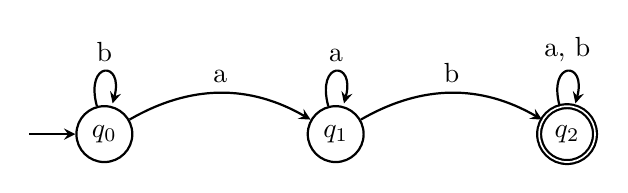
\begin{tikzpicture}[scale=1.2, >=stealth, node distance=2.2cm, thick]
          \node[circle, draw] (q0) {$q_0$};
          \node[circle, draw, right=of q0] (q1) {$q_1$};
          \node[circle, draw, double, right=of q1] (q2) {$q_2$};
          
          % Start arrow
          \draw[<-] (q0) -- (-0.8,0);
          
          % Transitions
          \path[->] 
            (q0) edge[bend left] node[above] {a} (q1)
            (q0) edge[loop above] node[above] {b} (q0)
            (q1) edge[loop above] node[above] {a} (q1)
            (q1) edge[bend left] node[above] {b} (q2)
            (q2) edge[loop above] node[above] {a, b} (q2);
        \end{tikzpicture}
        \end{center}
        This completes the design.
        
  \item \textbf{Subset Construction Example.}
  
        An NFA has states $Q = \{1, 2\}$, alphabet $\Sigma = \{a\}$, start state $1$, accept state $F = \{2\}$, and transitions:
        $\delta(1, a) = \{1, 2\}$, $\delta(2, a) = \emptyset$.
        Convert this NFA to an equivalent DFA using subset construction.
        
        \textbf{Solution:}
        In subset construction, each state of the new DFA corresponds to a subset of states of the NFA.
        1. **Start State:** The DFA start state is the subset of NFA states reachable from the start state $1$ using only $\epsilon$-transitions. Since there are no $\epsilon$-transitions, the start state is $\{1\}$.
        2. **Determine transitions:**
           For each DFA state (subset), we determine where the transition maps:
           * **From $\{1\}$:**
             \[
               \delta_{\text{DFA}}(\{1\}, a) \;=\; \delta_{\text{NFA}}(1, a) \;=\; \{1, 2\}.
             \]
             This creates a new DFA state: $\{1, 2\}$.
           * **From $\{1, 2\}$:**
             \[
               \delta_{\text{DFA}}(\{1, 2\}, a) \;=\; \delta_{\text{NFA}}(1, a) \cup \delta_{\text{NFA}}(2, a) \;=\; \{1, 2\} \cup \emptyset \;=\; \{1, 2\}.
             \]
             This maps back to $\{1, 2\}$.
           * **The empty set $\emptyset$:** (Created if any transition leads to no states). In this case, we do not reach the empty set state.
        3. **Accept States:** Any DFA state (subset) that contains at least one NFA accept state is a DFA accept state.
           * $\{1\}$ does not contain 2 (Reject).
           * $\{1, 2\}$ contains 2 (Accept).
           
        Thus, the equivalent DFA has:
        * $Q_{\text{DFA}} = \{\{1\}, \{1, 2\}\}$.
        * Start State: $\{1\}$.
        * Accept State: $\{1, 2\}$.
        * Transitions:
          * $\delta_{\text{DFA}}(\{1\}, a) = \{1, 2\}$.
          * $\delta_{\text{DFA}}(\{1, 2\}, a) = \{1, 2\}$.
        This is a 2-state DFA.
\end{enumerate}
\end{problembox}

\newpage

% ─── Section: Problems ───────────────────────────────────────────────────────
\section{Part 6 --- Problems}

\begin{problembox}
\begin{enumerate}[label=\textbf{P\arabic*.}]
  \item \textbf{DFA for Binary Divisibility.}
  
        Design a DFA over the alphabet $\Sigma = \{0, 1\}$ that accepts a binary string if and only if the binary number it represents is divisible by 3.
        \begin{enumerate}[label=(\alph*)]
          \item Let the states represent the remainder of the number modulo 3: $q_0$ (remainder 0), $q_1$ (remainder 1), and $q_2$ (remainder 2).
                If we are in state $q$ (representing value $V \equiv q \pmod 3$) and read a new bit $x \in \{0, 1\}$, the new value is $V_{new} = 2V + x$.
                Use this to fill in the transition function table $\delta(q, x)$.
          \item Specify the start state and the set of accept states.
          \item Draw the state transition diagram.
        \end{enumerate}

  \item \textbf{Pumping Lemma Proofs of Non-Regularity.}
  
        Use the Pumping Lemma to prove that the following languages are not regular:
        \begin{enumerate}[label=(\alph*)]
          \item The language of palindromes over $\Sigma = \{0, 1\}$:
                \[
                  L \;=\; \{w \in \{0,1\}^* : w = w^R\},
                \]
                where $w^R$ is the reverse of $w$.
          \item The language of squares over $\Sigma = \{1\}$:
                \[
                  L \;=\; \{1^{n^2} : n \ge 0\}.
                \]
        \end{enumerate}
\end{enumerate}
\end{problembox}

\newpage

% ─── Section: Deep Problems ──────────────────────────────────────────────────
\section{Part 7 --- Deep Problems}

\begin{deepbox}
\begin{enumerate}[label=\textbf{D\arabic*.}]
  \item \textbf{State Minimization and the Myhill-Nerode Theorem.}
  
        For any language $L \subseteq \Sigma^*$, we define the **Myhill-Nerode equivalence relation** $\equiv_L$ on strings in $\Sigma^*$ by:
        \[
          x \;\equiv_L\; y \iff \text{for all } z \in \Sigma^*, \; (xz \in L \iff yz \in L).
        \]
        This relation partitions the infinite set of all strings $\Sigma^*$ into equivalence classes.
        
        \begin{enumerate}[label=(\alph*)]
          \item Prove that $\equiv_L$ is an equivalence relation (reflexive, symmetric, and transitive).
          \item The Myhill-Nerode Theorem states that $L$ is regular if and only if the number of equivalence classes of $\equiv_L$ (the index) is finite.
                Furthermore, this index is exactly the minimum number of states in any DFA that recognizes $L$.
                
                Let $L = \{w \in \{0,1\}^* : w \text{ has an even number of 0s}\}$.
                Identify the equivalence classes of $\equiv_L$ and find the minimum number of states of the minimal DFA.
          \item Use the Myhill-Nerode theorem to prove that $L = \{0^n 1^n : n \ge 0\}$ is not regular. (Show that for any $i \neq j$, the strings $0^i$ and $0^j$ belong to different equivalence classes, implying the index is infinite).
        \end{enumerate}

  \item \textbf{The Power of Nondeterminism (State Blow-up).}
  
        Nondeterminism allows a machine to make guess branches. Although NFAs and DFAs recognize the same languages, the NFA representation can be exponentially smaller.
        Consider the language over $\Sigma = \{0, 1\}$:
        \[
          L_k \;=\; \{w \in \{0,1\}^* : \text{the } k\text{-th symbol from the right is a } 1\}.
        \]
        \begin{enumerate}[label=(\alph*)]
          \item Design an NFA with only $k+1$ states that recognizes $L_k$. (Use nondeterminism to guess when it is reading the $k$-th symbol from the right).
          \item Prove that any DFA that recognizes $L_k$ must have at least $2^k$ states. \textit{Hint: Show that for any two distinct binary strings $x$ and $y$ of length $k$, they must lead to different states in the DFA because there exists some suffix of length $< k$ that distinguishes them.}
          \item What does this exponential state space blow-up ($2^k$) reveal about the physical cost of turning a nondeterministic guess into a deterministic, step-by-step physical circuit?
        \end{enumerate}
\end{enumerate}
\end{deepbox}

\newpage

% ─── Section: Reflection ─────────────────────────────────────────────────────
\section{Part 8 --- Reflection}

\begin{reflectionbox}
\textbf{Conceptual Reflection}

Consider the following questions:
\begin{enumerate}
  \item **On the Pigeonhole Principle:** The Pumping Lemma is a direct consequence of the Pigeonhole Principle. How does this simple counting argument place an absolute physical limit on what a machine with a finite number of physical configurations (states) can calculate?
  \item **On Nondeterminism in Code:** An NFA can "guess" and branch. In a physical computer, we cannot branch infinitely without replicating hardware. How do we implement this "nondeterminism" in software? (Think about backtracking algorithms or subset simulation).
  \item **On the Boundaries of Regularity:** Regular expressions are used for string matching in programming. If a parser attempts to match HTML tags (which require matching pairs of open and close tags, like `<div>...</div>`), why does regular expression parser fail or crash if the tags are nested arbitrarily deep?
\end{enumerate}
\end{reflectionbox}

\medskip
\noindent\textbf{Looking ahead.}
Module~3.2 introduces **Context-Free Languages and Pushdown Automata**. Having proved that finite automata cannot count because their state space is finite, we will equip the machine with an infinite stack memory. We will study Context-Free Grammars and explore how this stack memory allows the machine to recognize nested structures.

\vspace{1.4cm}
\begin{center}
{\color{JourneyColor}\rule{0.5\linewidth}{0.8pt}}\\[6pt]
{\small\color{JourneyColor}\textit{End of Journey 3, Module 3.1 --- Finite Automata and Regular Languages}}\\[4pt]
{\small\color{JourneyColor}Continue to: \textbf{Module 3.2 --- Context-Free Languages and Pushdown Automata}}\\[6pt]
{\color{JourneyColor}\rule{0.5\linewidth}{0.8pt}}
\end{center}

\end{document}
